%==============================================================================
%  MATH 231 -- Linear Algebra I (Queens College, Fall 2026)
%  MATRIX UNIT, PART 3 -- Matrices That Move the Plane
%
%  Section numbering runs CONTINUOUSLY across the parts of the matrix unit;
%  see Part 2's header for the full map.  This part is Sections 15-21, hence
%  \setcounter{section}{14}.
%
%  STATUS: complete.  Sections 15-21.  Written from the plan in
%  plan/MATH231_remaining_units_plan.tex (2026-10-25).
%
%  AUDIENCE: distributed to students.  No instructor-facing apparatus.
%
%  WHAT THE INSTRUCTOR SPECIFIED, AND WHERE IT IS.
%   - Each action's matrix "derived and constructed from first principles":
%     every matrix in Sec. 16-19 is built from where the action sends e_1 and
%     e_2 (the recipe of Sec. 13.3, restated in Sec. 15.1), then read back
%     from its structure.
%   - The orthogonal-matrix derivation, in the instructor's order: the
%     question ||Ax|| = ||x||; Lemma 20.1 (symmetric M with x'Mx = 0 for all
%     x is zero, proved with x = e_i and x = e_i + e_j); x'(A'A - I)x = 0 and
%     the lemma give A'A = I (Theorem 20.2); orthonormal columns (Sec. 20.5);
%     the definition A'A = AA' = I with no inverse mentioned (Sec. 20.6).
%
%  DECISIONS CARRIED FROM THE PLAN.
%
%   D2. TRANSLATION IS NOT LINEAR.  The instructor's list puts translation
%       among the 2x2 actions.  No matrix acting on R^2 translates, because
%       A0 = 0.  Sec. 17 proves that, then performs translation with a 3x3
%       matrix in homogeneous coordinates, and shows composing it with a 2x2
%       action.  If translation is dropped, delete Sec. 17 whole; nothing later
%       depends on it except one remark at the end of the course.
%
%   D3. The derivation yields A'A = I only.  The definition (Sec. 20.6) keeps
%       both equations as specified.  For 2x2, Sec. 21.2 shows AA' = I follows
%       from A'A = I by direct computation; for n x n the general fact is
%       proved in Sec. 51.3, and Sec. 20.6 says so.
%
%   D9. The Kronecker delta is restated in Sec. 20.5 (it was introduced in
%       computational unit Sec. 16.2, which may not have been lectured).
%
%   D11. Composition.  Sec. 15.4 reads AB as "B first, then A", justified by
%       associativity M1 alone: (AB)x = A(Bx).  The derivation of the product
%       rule FROM composition is left to the end of the course.
%
%  REMARK AFTER LEMMA 20.1: the 90-degree rotation J has x'Jx = 0 for every
%  x, so symmetry cannot be dropped.  It ties to Homework 3 B.3
%  (skew-symmetric), but the document does not cite homework.
%
%  FIGURES: \actionpic{p}{q}{r}{s} draws the image of the unit square and of
%  an asymmetric letter F under [p q; r s], via cm={p,r,q,s,(0,0)} (tikz's
%  cm takes the COLUMNS).  Arrows for A e_1 (red) and A e_2 (green) are drawn
%  by hand after each call, so a zero column can be shown as a dot.
%
%  Compile with pdflatex or tectonic (standard TeX Live packages only; uses
%  tikz).
%==============================================================================
\documentclass[11pt]{article}

\usepackage[margin=1in]{geometry}
\usepackage{amsmath,amssymb,amsthm}
\usepackage[dvipsnames]{xcolor}
\usepackage{enumitem}
\usepackage{booktabs}
\usepackage{array}
\usepackage[hidelinks]{hyperref}
\usepackage{titlesec}
\usepackage{needspace}
\usepackage{tikz}
\usetikzlibrary{arrows.meta}

%------------------------------------------------------------------ style ----
\titleformat{\section}{\large\bfseries\sffamily}{\thesection.}{0.6em}{}
\titleformat{\subsection}{\normalsize\bfseries\sffamily}{\thesubsection.}{0.5em}{}
\titlespacing*{\section}{0pt}{14pt}{6pt}
\setlength{\emergencystretch}{3em}

\theoremstyle{plain}
\newtheorem{thm}{Theorem}[section]
\newtheorem{lem}[thm]{Lemma}
\newtheorem{cor}[thm]{Corollary}

\theoremstyle{definition}
\newtheorem{defn}{Definition}[section]
\newtheorem{ex}{Example}[section]
\theoremstyle{remark}
\newtheorem*{rmk}{Remark}
\newtheorem*{warn}{A common confusion}

\newcommand{\lookahead}{\par\smallskip\noindent
  \textbf{\sffamily\textcolor{RoyalBlue}{Looking ahead.}}\ \ignorespaces}
\newcommand{\lookback}[1][the vector unit]{\par\smallskip\noindent
  \textbf{\sffamily\textcolor{ForestGreen}{From #1.}}\ \ignorespaces}

%--------------------------------------------------------------- notation ----
\newcommand{\R}{\mathbb{R}}
\newcommand{\vc}[1]{\mathbf{#1}}
\newcommand{\mt}[1]{\mathbf{#1}}
\newcommand{\norm}[1]{\lVert #1\rVert}
\newcommand{\T}{^{\mathsf{T}}}
\newcommand{\colsp}[1]{\operatorname{col}[#1]}
\DeclareMathOperator{\spanop}{span}
\DeclareMathOperator{\diagop}{diag}
\DeclareMathOperator{\rank}{rank}

%------------------------------------------------------------- tikz helpers --
\tikzset{
  vecarr/.style   = {-{Stealth[length=2.6mm,width=2.0mm]},very thick},
  thinarr/.style  = {-{Stealth[length=2.2mm,width=1.7mm]},thick},
  axisline/.style = {->,gray!75,thin}
}
\newcommand{\Fshape}{(0.15,0.1) -- (0.35,0.1) -- (0.35,0.45) -- (0.65,0.45)
  -- (0.65,0.6) -- (0.35,0.6) -- (0.35,0.75) -- (0.8,0.75) -- (0.8,0.9)
  -- (0.15,0.9) -- cycle}
% \actionpic{p}{q}{r}{s}: the image of the unit square and of the F under the
% matrix [p q; r s], on a grid from -2.2 to 2.4.
\newcommand{\actionpic}[4]{%
  \begin{scope}
    \clip (-2.2,-2.2) rectangle (2.4,2.4);
    \draw[step=1cm,gray!22,very thin] (-3,-3) grid (3,3);
  \end{scope}
  \draw[axisline] (-2.2,0) -- (2.6,0);
  \draw[axisline] (0,-2.2) -- (0,2.6);
  \draw[gray!55,dashed] (0,0) -- (1,0) -- (1,1) -- (0,1) -- cycle;
  \fill[gray!30] \Fshape;
  \begin{scope}[cm={#1,#3,#2,#4,(0,0)}]
    \fill[RoyalBlue!15] (0,0) -- (1,0) -- (1,1) -- (0,1) -- cycle;
    \draw[RoyalBlue!60] (0,0) -- (1,0) -- (1,1) -- (0,1) -- cycle;
    \fill[RoyalBlue!75] \Fshape;
  \end{scope}}
\newcommand{\eone}[2]{\draw[vecarr,BrickRed] (0,0) -- (#1,#2);}
\newcommand{\etwo}[2]{\draw[vecarr,ForestGreen] (0,0) -- (#1,#2);}
\newcommand{\piclabel}[1]{\node[font=\small,align=center,anchor=north] at (0.1,-2.45) {#1};}
\newcommand{\smat}[1]{\left[\begin{smallmatrix}#1\end{smallmatrix}\right]}

\title{\vspace{-1.2cm}\textbf{\sffamily MATH 231 -- Linear Algebra I}\\[4pt]
       {\large\sffamily The Matrix Unit, Part 3 \textbullet\ Matrices That
        Move the Plane}\\[2pt]
       {\normalsize\sffamily Kiely Hall 326 \textbullet\
        Instructor: Kevin Bedoya}}
\author{}
\date{}

\begin{document}
\setcounter{section}{14}  % this part opens at Section 15; see the header note
\maketitle
\vspace{-1.6cm}

\noindent\textbf{About this document.} This is Part 3 of the matrix unit,
Sections 15--21. Section numbers run continuously through the unit, so \S13.3
points into Part 2. References into the vector unit always name it.

\medskip
\noindent\textbf{Assumed.} From Part 2: a matrix as a linear transformation,
and the fact that column $j$ of $\mt{A}$ is $\mt{A}\vc{e}_j$ (\S13); the
$2\times2$ determinant as an area factor with a sign (\S14). From Part 1: the
transpose and its laws (\S6.4), symmetric matrices (\S6.5), the norm written as
$\vc{v}\T\vc{v}$ (\S7.3), and M1--M6 (\S8.4). From the vector unit: length,
angle, the dot product, and orthogonality (\S10--\S11).

\medskip
\noindent\textbf{What you should be able to do afterwards.} Build the matrix of
a scaling, a shear, a rotation by a right angle, a reflection across an axis or
a diagonal, and a projection onto an axis, from where it sends $\vc{e}_1$ and
$\vc{e}_2$; recognise each from the structure of its matrix; explain why no
$2\times2$ matrix can translate, and translate with a $3\times3$ matrix instead;
prove that a matrix preserving every length satisfies
$\mt{A}\T\mt{A}=\mt{I}$; state what an orthogonal matrix is; and show that every
$2\times2$ orthogonal matrix is a rotation or a reflection.

%==============================================================================
\section{Building a matrix from what it does}
%==============================================================================

%------------------------------------------------------------------------------
\subsection{The recipe}
%------------------------------------------------------------------------------
\lookback[Part 2] A linear transformation of $\R^{2}$ is completely determined
by where it sends $\vc{e}_1$ and $\vc{e}_2$, and its matrix has those two images
as its columns (\S13.3). That turns a geometric description into a matrix in
three steps.

\begin{enumerate}[label=\textbf{Step \arabic*.},leftmargin=4.2em,itemsep=3pt]
  \item Decide, from the picture, where the motion sends $\vc{e}_1=[\,1,0\,]$.
  \item Decide where it sends $\vc{e}_2=[\,0,1\,]$.
  \item Write those two vectors down as the first and second columns.
\end{enumerate}

\noindent Every matrix in \S16--\S19 is built this way, and nothing else is
needed, \emph{provided the motion is linear}. That proviso is not automatic, so
it is worth knowing how to spot a motion that fails it.

%------------------------------------------------------------------------------
\subsection{Is the motion linear?}
%------------------------------------------------------------------------------
From \S13.2 and \S13.4, a linear transformation of the plane
\begin{itemize}[leftmargin=1.4em,itemsep=2pt]
  \item keeps the origin where it is;
  \item sends lines through the origin to lines through the origin (or to the
        origin itself);
  \item sends the coordinate grid to a grid whose lines are still parallel and
        still evenly spaced.
\end{itemize}
A motion that breaks any of these is not linear, and no matrix performs it.
Bending a line into a curve breaks the second; any motion that moves the origin
breaks the first. \S17 is about the most natural motion of that kind.

%------------------------------------------------------------------------------
\subsection{Reading the structure back}
%------------------------------------------------------------------------------
The recipe also runs backwards. Given a matrix, its columns say where
$\vc{e}_1$ and $\vc{e}_2$ go, and the \emph{pattern} of its entries (\S4) says
what kind of motion it is. The one pattern to watch from the start is the
off-diagonal. In
\[
  \begin{bmatrix}a&b\\c&d\end{bmatrix}
  \begin{bmatrix}x\\y\end{bmatrix}
  =\begin{bmatrix}ax+by\\cx+dy\end{bmatrix},
\]
the off-diagonal entries $b$ and $c$ are the only ones that let $y$ influence
the new first coordinate, or $x$ the new second one. A diagonal matrix keeps
the two coordinates separate. Every matrix with nonzero off-diagonal entries
mixes them.

%------------------------------------------------------------------------------
\subsection{One motion after another}
%------------------------------------------------------------------------------
Two motions can be done in succession: first $\mt{B}$, then $\mt{A}$. The point
$\vc{x}$ goes first to $\mt{B}\vc{x}$, then to $\mt{A}(\mt{B}\vc{x})$. By
associativity (M1 of \S8.4, with $\vc{x}$ read as an $n\times1$ matrix),
\[
  \mt{A}(\mt{B}\vc{x}) \;=\; (\mt{A}\mt{B})\vc{x} .
\]
So \emph{the matrix of ``first $\mt{B}$, then $\mt{A}$'' is the product
$\mt{A}\mt{B}$.} Mind the order: the motion done first is written on the
\emph{right}, next to the vector it acts on. Since $\mt{A}\mt{B}$ and
$\mt{B}\mt{A}$ are usually different (\S8.4), the order in which motions are
done usually matters.

\noindent In the figures below, the dashed square and the grey F are the
starting position. The shaded parallelogram and the blue F are where the
matrix moves them. The red arrow is $\mt{A}\vc{e}_1$ and the green arrow is
$\mt{A}\vc{e}_2$, which are the two columns.

%==============================================================================
\section{Scaling}
%==============================================================================

%------------------------------------------------------------------------------
\subsection{Uniform scaling}
%------------------------------------------------------------------------------
\emph{The motion:} stretch every vector by the same factor $\alpha$, so
$\vc{x}\mapsto\alpha\vc{x}$.

\emph{The recipe:} $\vc{e}_1\mapsto\alpha\vc{e}_1=[\,\alpha,0\,]$ and
$\vc{e}_2\mapsto\alpha\vc{e}_2=[\,0,\alpha\,]$. So the matrix is
\[
  \begin{bmatrix}\alpha&0\\0&\alpha\end{bmatrix} \;=\; \alpha\mt{I},
  \qquad
  \alpha\mt{I}\,\vc{x}=\alpha\vc{x}. \quad\checkmark
\]

\noindent Every vector stays on its own line through the origin, and every
length is multiplied by $|\alpha|$. With $\alpha>1$ the plane is enlarged; with
$0<\alpha<1$ it shrinks; with $\alpha=0$ it collapses to the origin. With
$\alpha<0$ every vector is also turned to point the opposite way, and
$\alpha=-1$ gives $-\mt{I}$, which \S19 identifies as a rotation by
$180^\circ$.

The determinant is $\det(\alpha\mt{I})=\alpha\cdot\alpha-0=\alpha^{2}$. Doubling
every length multiplies every area by $4$, which is the familiar rule for
similar figures, now read off a matrix.

%------------------------------------------------------------------------------
\subsection{Non-uniform scaling}
%------------------------------------------------------------------------------
\emph{The motion:} stretch the $x$-direction by $s_1$ and the $y$-direction by
$s_2$, independently: $[\,x,y\,]\mapsto[\,s_1x,\ s_2y\,]$.

\emph{The recipe:} $\vc{e}_1\mapsto[\,s_1,0\,]$ and
$\vc{e}_2\mapsto[\,0,s_2\,]$, so the matrix is the diagonal matrix
\[
  \diagop(s_1,s_2)=\begin{bmatrix}s_1&0\\0&s_2\end{bmatrix},
  \qquad
  \det=s_1s_2 .
\]

\noindent A circle becomes an ellipse. If $[\,x,y\,]$ is on the unit circle,
$x^{2}+y^{2}=1$, then its image $[\,u,v\,]=[\,s_1x,\,s_2y\,]$ satisfies
\[
  \frac{u^{2}}{s_1^{2}}+\frac{v^{2}}{s_2^{2}} \;=\; x^{2}+y^{2} \;=\; 1 ,
\]
an ellipse with semi-axes $|s_1|$ and $|s_2|$ along the coordinate axes.
A negative entry also reverses one direction: $\diagop(-1,1)$ sends
$[\,x,y\,]$ to $[\,-x,y\,]$, the mirror image across the $y$-axis, and its
determinant is $-1$.

\begin{center}
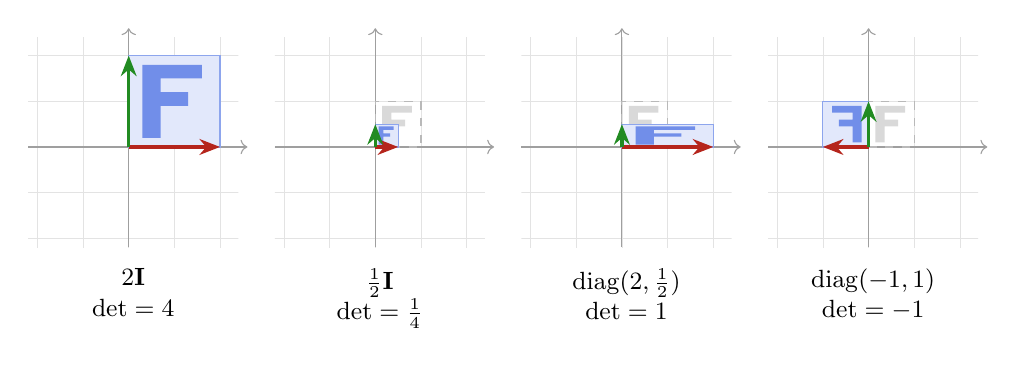
\begin{tikzpicture}[scale=0.58]
  \actionpic{2}{0}{0}{2}
  \eone{2}{0}\etwo{0}{2}
  \piclabel{$2\mt{I}$\\ $\det=4$}
  \begin{scope}[xshift=5.4cm]
    \actionpic{0.5}{0}{0}{0.5}
    \eone{0.5}{0}\etwo{0}{0.5}
    \piclabel{$\tfrac12\mt{I}$\\ $\det=\tfrac14$}
  \end{scope}
  \begin{scope}[xshift=10.8cm]
    \actionpic{2}{0}{0}{0.5}
    \eone{2}{0}\etwo{0}{0.5}
    \piclabel{$\diagop(2,\tfrac12)$\\ $\det=1$}
  \end{scope}
  \begin{scope}[xshift=16.2cm]
    \actionpic{-1}{0}{0}{1}
    \eone{-1}{0}\etwo{0}{1}
    \piclabel{$\diagop(-1,1)$\\ $\det=-1$}
  \end{scope}
\end{tikzpicture}
\end{center}

\noindent The third picture is worth a second look: stretched by $2$ one way
and squeezed by $\tfrac12$ the other, the square changes shape completely and
keeps its area exactly, as $\det=1$ says.

%------------------------------------------------------------------------------
\subsection{The structure: diagonal}
%------------------------------------------------------------------------------
A matrix is diagonal (\S4.2) exactly when $\mt{A}\vc{e}_1$ is a multiple of
$\vc{e}_1$ and $\mt{A}\vc{e}_2$ is a multiple of $\vc{e}_2$, that is, when each
coordinate axis is sent into itself. Diagonal matrices are the scalings, and the
zeros off the diagonal are the statement that the coordinates are not mixed.

%==============================================================================
\section{Translation}
%==============================================================================

%------------------------------------------------------------------------------
\subsection{The motion}
%------------------------------------------------------------------------------
Slide the whole plane by a fixed vector $\vc{t}=[\,t_1,t_2\,]$, so
$\vc{x}\mapsto\vc{x}+\vc{t}$. Nothing turns, nothing stretches: every point
moves the same distance in the same direction. It is the simplest motion there
is.

%------------------------------------------------------------------------------
\subsection{No \texorpdfstring{$2\times2$}{2x2} matrix does it}
%------------------------------------------------------------------------------
\begin{thm}
\label{thm:notranslate}
If $\vc{t}\neq\vc{0}$, there is no matrix $\mt{A}\in\R^{2\times2}$ with
$\mt{A}\vc{x}=\vc{x}+\vc{t}$ for every $\vc{x}\in\R^{2}$.
\end{thm}

\begin{proof}
Try $\vc{x}=\vc{0}$. Every matrix sends $\vc{0}$ to $\vc{0}$, since each entry
of $\mt{A}\vc{0}$ is a dot product with the zero vector. The translation sends
$\vc{0}$ to $\vc{t}\neq\vc{0}$.
\end{proof}

\noindent Translation fails the first test of \S15.2: it moves the origin. It
fails the definition of linearity too, since doubling the input does not double
the output: $2\vc{x}+\vc{t}\neq2(\vc{x}+\vc{t})$. Applying the recipe of
\S15.1 anyway would put $\vc{e}_1+\vc{t}$ and $\vc{e}_2+\vc{t}$ in as columns,
and the resulting matrix still sends $\vc{0}$ to $\vc{0}$, so it is not the
translation. That is the mistake the proviso in \S15.1 guards against.

%------------------------------------------------------------------------------
\subsection{Homogeneous coordinates}
%------------------------------------------------------------------------------
There is a way around this, and it is used by every computer graphics system:
add a third coordinate, always equal to $1$. Represent the point $[\,x,y\,]$ of
the plane by $[\,x,y,1\,]\in\R^{3}$. Then
\[
  \begin{bmatrix} 1&0&t_1\\ 0&1&t_2\\ 0&0&1 \end{bmatrix}
  \begin{bmatrix} x\\ y\\ 1 \end{bmatrix}
  =
  \begin{bmatrix} x+t_1\\ y+t_2\\ 1 \end{bmatrix} .
\]
The first two entries are the translated point, and the third is still $1$. A
translation of the plane has become multiplication by a $3\times3$ matrix. The
origin of $\R^{3}$ still stays put, as it must. What moves is the origin of
the \emph{plane}, which now lives at $[\,0,0,1\,]$.

\begin{rmk}
Seen in $\R^{3}$, that matrix is a shear (\S18): it slides each horizontal
slice $z=c$ sideways by $c\,\vc{t}$, and the plane $z=1$, where our copy of
$\R^{2}$ lives, by exactly $\vc{t}$. A motion that is not linear in two
dimensions becomes linear one dimension up.
\end{rmk}

%------------------------------------------------------------------------------
\subsection{Combining translation with the other motions}
%------------------------------------------------------------------------------
Any $2\times2$ matrix $\mt{M}$ fits into the same scheme as the block matrix
$\begin{bmatrix}\mt{M}&\vc{0}\\\vc{0}\T&1\end{bmatrix}$, which applies
$\mt{M}$ to $[\,x,y\,]$ and leaves the $1$ alone. Then motions of both kinds can
be chained by multiplying $3\times3$ matrices, in the order of \S15.4.

\begin{ex}
Rotate by $90^\circ$ (the matrix $\mt{J}$ of \S19.1) and \emph{then} translate
by $\vc{t}=[\,2,0\,]$. The second motion is written on the left:
\[
  \begin{bmatrix}1&0&2\\0&1&0\\0&0&1\end{bmatrix}
  \begin{bmatrix}0&-1&0\\1&0&0\\0&0&1\end{bmatrix}
  =
  \begin{bmatrix}0&-1&2\\1&0&0\\0&0&1\end{bmatrix}.
\]
On the point $[\,2,0\,]$: rotating gives $[\,0,2\,]$, translating gives
$[\,2,2\,]$, and the matrix agrees:
$[\,0-0+2,\ 2+0+0,\ 1\,]=[\,2,2,1\,]$. In the other order, translate first and
then rotate, the product is
$\begin{bmatrix}0&-1&0\\1&0&2\\0&0&1\end{bmatrix}$. That is a different motion,
as \S15.4 warned.
\end{ex}

%==============================================================================
\section{Shear}
%==============================================================================

%------------------------------------------------------------------------------
\subsection{The horizontal shear}
%------------------------------------------------------------------------------
\emph{The motion:} hold the $x$-axis fixed and slide every horizontal line
sideways by an amount proportional to its height. A deck of cards pushed from
the side does this.

\emph{The recipe:} $\vc{e}_1$ is on the $x$-axis and stays put. $\vc{e}_2$ is
at height $1$, so it slides sideways by $k$ to $[\,k,1\,]$. The matrix is
\[
  \mt{S}=\begin{bmatrix}1&k\\0&1\end{bmatrix},
  \qquad
  \mt{S}\begin{bmatrix}x\\y\end{bmatrix}=\begin{bmatrix}x+ky\\y\end{bmatrix}.
\]
A point at height $y$ moves sideways by $ky$, as described.

%------------------------------------------------------------------------------
\subsection{The vertical shear}
%------------------------------------------------------------------------------
Holding the $y$-axis fixed instead and sliding vertical lines up by $k$ times
their distance across gives $\vc{e}_1\mapsto[\,1,k\,]$, $\vc{e}_2\mapsto\vc{e}_2$,
and the matrix $\begin{bmatrix}1&0\\k&1\end{bmatrix}$, the transpose of the
horizontal shear.

\begin{center}
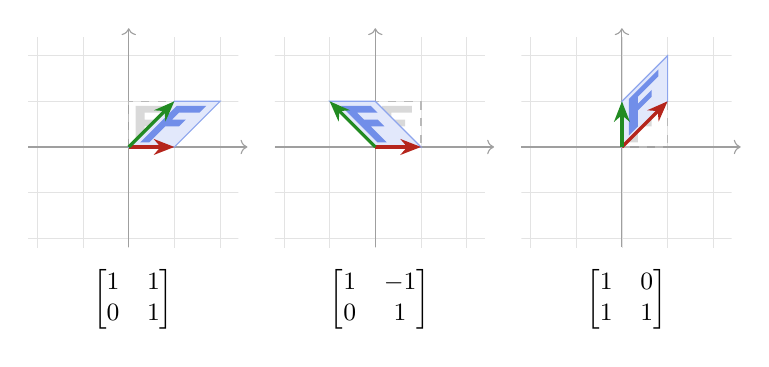
\begin{tikzpicture}[scale=0.58]
  \actionpic{1}{1}{0}{1}
  \eone{1}{0}\etwo{1}{1}
  \piclabel{$\begin{bmatrix}1&1\\0&1\end{bmatrix}$}
  \begin{scope}[xshift=5.4cm]
    \actionpic{1}{-1}{0}{1}
    \eone{1}{0}\etwo{-1}{1}
    \piclabel{$\begin{bmatrix}1&-1\\0&1\end{bmatrix}$}
  \end{scope}
  \begin{scope}[xshift=10.8cm]
    \actionpic{1}{0}{1}{1}
    \eone{1}{1}\etwo{0}{1}
    \piclabel{$\begin{bmatrix}1&0\\1&1\end{bmatrix}$}
  \end{scope}
\end{tikzpicture}
\end{center}

%------------------------------------------------------------------------------
\subsection{The structure, and the area}
%------------------------------------------------------------------------------
A shear is triangular (\S4.4) with $1$s on the diagonal, and
$\det\mt{S}=1\cdot1-k\cdot0=1$. The area is unchanged, and the picture says
why: the square becomes a parallelogram with the same base and the same height.
Lengths and angles do change. $\vc{e}_2$, of length $1$, becomes $[\,k,1\,]$, of
length $\sqrt{1+k^{2}}$. A shear changes shape without changing area.

%==============================================================================
\section{Rotation, reflection and projection: first examples}
%==============================================================================
Three more kinds of motion, each met here in its simplest form. The rotation by
a general angle is built in \S24, and the projection onto a general line in
\S26.

%------------------------------------------------------------------------------
\subsection{Rotation by a right angle}
%------------------------------------------------------------------------------
\emph{The motion:} turn the plane a quarter-turn counterclockwise about the
origin.

\emph{The recipe:} $\vc{e}_1=[\,1,0\,]$, pointing east, turns to point north:
$[\,0,1\,]$. $\vc{e}_2=[\,0,1\,]$, pointing north, turns to point west:
$[\,-1,0\,]$. So
\[
  \mt{J}=\begin{bmatrix}0&-1\\1&0\end{bmatrix},
  \qquad
  \mt{J}\begin{bmatrix}x\\y\end{bmatrix}=\begin{bmatrix}-y\\x\end{bmatrix}.
\]
A check that this really is a quarter-turn: $[\,x,y\,]$ and $[\,-y,x\,]$ have
the same length, and their dot product is $-xy+yx=0$, so they are orthogonal.

\begin{rmk}
Compare the complex numbers: multiplying $x+iy$ by $i$ gives $-y+ix$, the same
arithmetic. Multiplication by $i$ is a quarter-turn of the complex plane, and
$\mt{J}$ is its matrix.
\end{rmk}

\noindent A half-turn sends $\vc{e}_1\mapsto-\vc{e}_1$ and $\vc{e}_2\mapsto-\vc{e}_2$,
which is $-\mt{I}$, the uniform scaling by $-1$ of \S16.1 seen from another
angle. And two quarter-turns make a half-turn: by \S15.4 that is
$\mt{J}\mt{J}=\mt{J}^{2}$, and indeed
$\mt{J}^{2}=\begin{bmatrix}0&-1\\1&0\end{bmatrix}\begin{bmatrix}0&-1\\1&0\end{bmatrix}
=\begin{bmatrix}-1&0\\0&-1\end{bmatrix}=-\mt{I}$, the matrix version of
$i^{2}=-1$.

%------------------------------------------------------------------------------
\subsection{Reflections}
%------------------------------------------------------------------------------
\emph{Across the $x$-axis:} $\vc{e}_1$ is on the mirror and stays;
$\vc{e}_2$ flips to $-\vc{e}_2$. The matrix is $\diagop(1,-1)$, and
$[\,x,y\,]\mapsto[\,x,-y\,]$. Across the $y$-axis it is $\diagop(-1,1)$, as in
\S16.2.

\emph{Across the line $y=x$:} the mirror makes a $45^\circ$ angle with each
axis, so it swaps them: $\vc{e}_1\mapsto\vc{e}_2$ and $\vc{e}_2\mapsto\vc{e}_1$.
\[
  \begin{bmatrix}0&1\\1&0\end{bmatrix},
  \qquad
  [\,x,y\,]\mapsto[\,y,x\,] .
\]
The reflection across $y=x$ simply exchanges the two coordinates. Across the
other diagonal, $y=-x$, the same reasoning gives
$\vc{e}_1\mapsto-\vc{e}_2$, $\vc{e}_2\mapsto-\vc{e}_1$, and
$\begin{bmatrix}0&-1\\-1&0\end{bmatrix}$.

Each reflection has determinant $-1$: it turns the plane over. And each one,
done twice, puts everything back. For example,
$\begin{bmatrix}0&1\\1&0\end{bmatrix}^{2}=\mt{I}$.

%------------------------------------------------------------------------------
\subsection{Projection onto an axis}
%------------------------------------------------------------------------------
\emph{The motion:} drop every point straight down (or up) onto the $x$-axis:
$[\,x,y\,]\mapsto[\,x,0\,]$. Think of the shadow cast by a light directly
overhead.

\emph{The recipe:} $\vc{e}_1$ is already on the $x$-axis and stays;
$\vc{e}_2$ is straight above the origin and drops to $\vc{0}$. So
\[
  \mt{P}=\begin{bmatrix}1&0\\0&0\end{bmatrix}=\diagop(1,0) .
\]
This is the first matrix in the gallery with determinant $0$ and rank $1$
(\S14.2). The whole plane is flattened onto the $x$-axis, and the whole $y$-axis
is crushed to the origin. Projecting a second time changes nothing, since a
point already on the $x$-axis stays there, so $\mt{P}^{2}=\mt{P}$. Part 5 takes
that equation as the definition of a projection.

\begin{center}
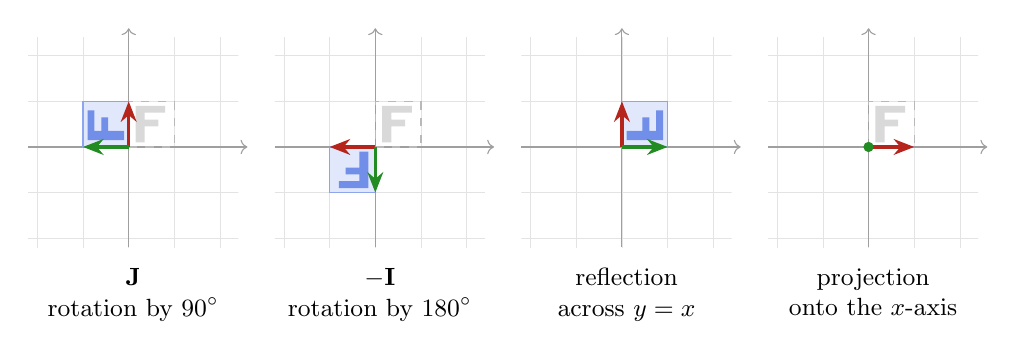
\begin{tikzpicture}[scale=0.58]
  \actionpic{0}{-1}{1}{0}
  \eone{0}{1}\etwo{-1}{0}
  \piclabel{$\mt{J}$\\ rotation by $90^\circ$}
  \begin{scope}[xshift=5.4cm]
    \actionpic{-1}{0}{0}{-1}
    \eone{-1}{0}\etwo{0}{-1}
    \piclabel{$-\mt{I}$\\ rotation by $180^\circ$}
  \end{scope}
  \begin{scope}[xshift=10.8cm]
    \actionpic{0}{1}{1}{0}
    \eone{0}{1}\etwo{1}{0}
    \piclabel{reflection\\ across $y=x$}
  \end{scope}
  \begin{scope}[xshift=16.2cm]
    \actionpic{1}{0}{0}{0}
    \eone{1}{0}
    \fill[ForestGreen] (0,0) circle (3.2pt);
    \piclabel{projection\\ onto the $x$-axis}
  \end{scope}
\end{tikzpicture}
\end{center}

\noindent In the last picture $\mt{P}\vc{e}_2=\vc{0}$, shown as the green dot,
and the F has been flattened into a segment of the $x$-axis.

%------------------------------------------------------------------------------
\subsection{The gallery so far}
%------------------------------------------------------------------------------
\begin{center}
\renewcommand{\arraystretch}{1.5}
\begin{tabular}{@{}l c c l@{}}
\toprule
\textbf{Motion} & \textbf{Matrix} & $\det$ & \textbf{Structure} \\
\midrule
uniform scaling by $\alpha$ & $\alpha\mt{I}$ & $\alpha^{2}$ & multiple of $\mt{I}$ \\
scaling the axes by $s_1,s_2$ & $\diagop(s_1,s_2)$ & $s_1s_2$ & diagonal \\
horizontal shear & $\smat{1&k\\0&1}$ & $1$ & triangular, unit diagonal \\
rotation by $90^\circ$ & $\smat{0&-1\\1&0}$ & $1$ & $\mt{J}\T=-\mt{J}$ \\
reflection across $y=x$ & $\smat{0&1\\1&0}$ & $-1$ & symmetric, swaps coordinates \\
projection onto the $x$-axis & $\diagop(1,0)$ & $0$ & diagonal, rank $1$ \\
translation by $\vc{t}\neq\vc{0}$ & none ($2\times2$) & --- & not linear \\
\bottomrule
\end{tabular}
\end{center}

%==============================================================================
\section{Matrices that preserve length}
%==============================================================================

%------------------------------------------------------------------------------
\subsection{The question}
%------------------------------------------------------------------------------
Some motions in the gallery change lengths and some do not. A scaling by $2$
doubles every length. A shear sends $\vc{e}_2$, of length $1$, to $[\,k,1\,]$,
of length $\sqrt{1+k^{2}}$. A projection sends $\vc{e}_2$ to $\vc{0}$. But the
quarter-turn $\mt{J}$ and the reflections move every vector without changing its
length at all. So we ask:

\begin{quote}
Which matrices $\mt{A}\in\R^{n\times n}$ satisfy
$\norm{\mt{A}\vc{x}}_2=\norm{\vc{x}}_2$ for every $\vc{x}\in\R^{n}$?
\end{quote}

\noindent The question makes sense in any dimension, and the answer will too.
Think of $n=2$ while reading.

%------------------------------------------------------------------------------
\subsection{Rewriting the condition}
%------------------------------------------------------------------------------
Lengths are awkward to work with because of the square root, so square both
sides. \S7.3 wrote the squared norm as a product: $\norm{\vc{v}}^{2}=\vc{v}\T\vc{v}$.
Applied to $\vc{v}=\mt{A}\vc{x}$, with $(\mt{A}\vc{x})\T=\vc{x}\T\mt{A}\T$ by
M6,
\[
  \norm{\mt{A}\vc{x}}^{2}=(\mt{A}\vc{x})\T(\mt{A}\vc{x})
  =\vc{x}\T\mt{A}\T\mt{A}\vc{x},
  \qquad
  \norm{\vc{x}}^{2}=\vc{x}\T\vc{x}=\vc{x}\T\mt{I}\vc{x}.
\]
So the condition $\norm{\mt{A}\vc{x}}^{2}=\norm{\vc{x}}^{2}$ for every $\vc{x}$
says, after subtracting and using distributivity,
\[
  \boxed{\;\vc{x}\T\bigl(\mt{A}\T\mt{A}-\mt{I}\bigr)\vc{x}=0
  \quad\text{for every }\vc{x}\in\R^{n}.\;}
\]
The expression $\vc{x}\T\mt{M}\vc{x}$ is a number (a $1\times n$ times an
$n\times n$ times an $n\times1$). The question has become: if a matrix
$\mt{M}$ makes this number zero for every $\vc{x}$, must $\mt{M}$ itself be
zero?

%------------------------------------------------------------------------------
\subsection{The lemma}
%------------------------------------------------------------------------------
One small computation does all the work. For standard basis vectors,
\[
  \vc{e}_i\T\mt{M}\vc{e}_j \;=\; m_{ij},
\]
because $\mt{M}\vc{e}_j$ is column $j$ of $\mt{M}$ (\S13.3), and dotting with
$\vc{e}_i$ picks out its $i$-th entry. So by feeding in well-chosen
vectors, the number $\vc{x}\T\mt{M}\vc{x}$ can be made to report individual
entries of $\mt{M}$.

\begin{lem}
\label{lem:quadzero}
Let $\mt{M}\in\R^{n\times n}$ be symmetric, $\mt{M}\T=\mt{M}$, and suppose
$\vc{x}\T\mt{M}\vc{x}=0$ for every $\vc{x}\in\R^{n}$. Then $\mt{M}=\mt{0}$.
\end{lem}

\begin{proof}
\emph{The diagonal.} Take $\vc{x}=\vc{e}_i$. Then
$0=\vc{e}_i\T\mt{M}\vc{e}_i=m_{ii}$. So every diagonal entry is zero.

\emph{Off the diagonal.} Take $i\neq j$ and $\vc{x}=\vc{e}_i+\vc{e}_j$.
Expanding with the distributive laws,
\[
  0=(\vc{e}_i+\vc{e}_j)\T\mt{M}(\vc{e}_i+\vc{e}_j)
   =\vc{e}_i\T\mt{M}\vc{e}_i+\vc{e}_i\T\mt{M}\vc{e}_j
    +\vc{e}_j\T\mt{M}\vc{e}_i+\vc{e}_j\T\mt{M}\vc{e}_j
   =m_{ii}+m_{ij}+m_{ji}+m_{jj} .
\]
The diagonal entries are already known to be $0$, and $m_{ji}=m_{ij}$ by
symmetry, so this says $2m_{ij}=0$. Hence $m_{ij}=0$ for every $i\neq j$ as
well.
\end{proof}

\noindent For $n=2$ the lemma can be seen in one line. Writing it out,
\[
  \vc{x}\T\mt{M}\vc{x}=m_{11}x_1^{2}+(m_{12}+m_{21})\,x_1x_2+m_{22}x_2^{2},
\]
and the proof chose $\vc{x}=[\,1,0\,]$, $[\,0,1\,]$ and $[\,1,1\,]$ to isolate
the three coefficients one at a time.

\begin{rmk}[Why symmetry is needed]
The display shows that $\vc{x}\T\mt{M}\vc{x}$ only ever sees the
\emph{sum} $m_{12}+m_{21}$, never the two entries separately. Without symmetry the
lemma is false. The quarter-turn of \S19.1 gives
\[
  \vc{x}\T\mt{J}\vc{x}
  =\begin{bmatrix}x_1&x_2\end{bmatrix}\begin{bmatrix}-x_2\\x_1\end{bmatrix}
  =-x_1x_2+x_2x_1=0
\]
for every $\vc{x}$, and $\mt{J}\neq\mt{0}$. Geometrically this says
$\mt{J}\vc{x}\perp\vc{x}$ for every $\vc{x}$, which is what a quarter-turn does.
Matrices like $\mt{J}$, with $\mt{M}\T=-\mt{M}$, are called
\emph{skew-symmetric}, and they are exactly the ones whose $\vc{x}\T\mt{M}\vc{x}$
is always zero. The proof above breaks at the step $m_{ij}+m_{ji}=0$, which for
them says only $m_{ji}=-m_{ij}$.
\end{rmk}

%------------------------------------------------------------------------------
\subsection{The theorem}
%------------------------------------------------------------------------------
\begin{thm}
\label{thm:lengthpres}
Let $\mt{A}\in\R^{n\times n}$. Then $\norm{\mt{A}\vc{x}}=\norm{\vc{x}}$ for every
$\vc{x}\in\R^{n}$ if and only if $\mt{A}\T\mt{A}=\mt{I}$.
\end{thm}

\begin{proof}
Suppose lengths are preserved. By \S20.2 the matrix
$\mt{M}=\mt{A}\T\mt{A}-\mt{I}$ has $\vc{x}\T\mt{M}\vc{x}=0$ for every
$\vc{x}$. It is symmetric: $(\mt{A}\T\mt{A})\T=\mt{A}\T(\mt{A}\T)\T=\mt{A}\T\mt{A}$
by M6 and $(\mt{A}\T)\T=\mt{A}$ (\S6.4), $\mt{I}$ is symmetric, and the
transpose of a difference is the difference of the transposes (\S6.4). So the
lemma applies, $\mt{M}=\mt{0}$, and $\mt{A}\T\mt{A}=\mt{I}$.

Conversely, if $\mt{A}\T\mt{A}=\mt{I}$ then
$\norm{\mt{A}\vc{x}}^{2}=\vc{x}\T\mt{A}\T\mt{A}\vc{x}=\vc{x}\T\vc{x}=\norm{\vc{x}}^{2}$.
\end{proof}

%------------------------------------------------------------------------------
\subsection{Reading \texorpdfstring{$\mt{A}\T\mt{A}=\mt{I}$}{A'A = I} column by column}
%------------------------------------------------------------------------------
The equation $\mt{A}\T\mt{A}=\mt{I}$ is $n^{2}$ equations, one per entry, and
each says something about the columns $\vc{a}_1,\dots,\vc{a}_n$ of $\mt{A}$.
Row $i$ of $\mt{A}\T$ is column $i$ of $\mt{A}$, so
\[
  (\mt{A}\T\mt{A})_{ij}
  =(\text{row } i \text{ of } \mt{A}\T)\cdot(\text{column } j \text{ of } \mt{A})
  =\vc{a}_i\T\vc{a}_j .
\]
The entries of $\mt{I}$ are recorded by the \textbf{Kronecker delta},
\[
  \delta_{ij}=\begin{cases}1 & i=j,\\ 0 & i\neq j,\end{cases}
\]
so $\mt{A}\T\mt{A}=\mt{I}$ says $\vc{a}_i\T\vc{a}_j=\delta_{ij}$ for every pair
$i,j$. Read in two halves:
\begin{itemize}[leftmargin=1.4em,itemsep=3pt]
  \item $i=j$: $\vc{a}_i\T\vc{a}_i=\norm{\vc{a}_i}^{2}=1$. \emph{Every column is
        a unit vector.}
  \item $i\neq j$: $\vc{a}_i\T\vc{a}_j=0$. \emph{Every two different columns
        are orthogonal.}
\end{itemize}

\begin{defn}[Orthonormal]
Vectors $\vc{q}_1,\dots,\vc{q}_k$ are \textbf{orthonormal} if
$\vc{q}_i\T\vc{q}_j=\delta_{ij}$: each has length $1$ and each two are
orthogonal.
\end{defn}

\begin{thm}
For $\mt{A}\in\R^{n\times n}$ the following are equivalent:
$\norm{\mt{A}\vc{x}}=\norm{\vc{x}}$ for every $\vc{x}$;
$\mt{A}\T\mt{A}=\mt{I}$; the columns of $\mt{A}$ are orthonormal.
\end{thm}

\noindent Orthogonal nonzero vectors are independent (the vector unit, \S21.2),
so $n$ orthonormal columns are an orthonormal \emph{basis} of $\R^{n}$. And
the converse direction of \S20.4 shows more than lengths survive. For any
$\vc{x},\vc{y}$,
\[
  (\mt{A}\vc{x})\T(\mt{A}\vc{y})=\vc{x}\T\mt{A}\T\mt{A}\vc{y}=\vc{x}\T\vc{y},
\]
so dot products are preserved, and with them angles (the vector unit, \S11.3).
A length-preserving matrix moves the space \emph{rigidly}: nothing is stretched,
nothing is bent, no angle opens or closes.

%------------------------------------------------------------------------------
\subsection{Orthogonal matrices}
%------------------------------------------------------------------------------
\begin{defn}[Orthogonal matrix]
A square matrix $\mt{A}\in\R^{n\times n}$ is \textbf{orthogonal} if
\[
  \mt{A}\T\mt{A}=\mt{A}\mt{A}\T=\mt{I} .
\]
\end{defn}

\noindent The first equation is the one \S20.4 derived; it says the columns are
orthonormal. The second says the \emph{rows} are orthonormal, by the same
computation applied to $\mt{A}\T$. For $2\times2$ matrices, \S21 shows that the
second equation follows from the first. It does for every square matrix, though
the proof needs the inverse matrix and comes in \S51.3. Once that is proved, an
orthogonal matrix is simply a square matrix with orthonormal columns, and the
rows come free.

\begin{warn}[``Orthogonal'' means orthonormal]
An orthogonal matrix has ortho\emph{normal} columns, not merely orthogonal
ones. $\diagop(2,1)$ has orthogonal columns, but it doubles the length of
$\vc{e}_1$, so it is not an orthogonal matrix. The name is a historical accident,
and it has stuck.
\end{warn}

\begin{ex}
From the gallery:
\[
  \mt{J}\T\mt{J}
  =\begin{bmatrix}0&1\\-1&0\end{bmatrix}\begin{bmatrix}0&-1\\1&0\end{bmatrix}
  =\begin{bmatrix}1&0\\0&1\end{bmatrix},
\]
and $\mt{J}\mt{J}\T=\mt{I}$ likewise, so $\mt{J}$ is orthogonal. So are
$-\mt{I}$, $\diagop(1,-1)$, and $\begin{bmatrix}0&1\\1&0\end{bmatrix}$: each has
columns that are unit vectors at right angles. The scaling $2\mt{I}$, the shear
and the projection $\diagop(1,0)$ are not.
\end{ex}

%==============================================================================
\section{What an orthogonal matrix can do}
%==============================================================================
In the plane, the condition ``orthonormal columns'' is restrictive enough to
list every possibility.

%------------------------------------------------------------------------------
\subsection{The second column is nearly determined by the first}
%------------------------------------------------------------------------------
\begin{lem}
\label{lem:perp}
Let $[\,a,c\,]\neq\vc{0}$. The vectors of $\R^{2}$ orthogonal to $[\,a,c\,]$
are exactly the multiples of $[\,-c,a\,]$.
\end{lem}

\begin{proof}
First, $[\,-c,a\,]\cdot[\,a,c\,]=-ca+ac=0$, so every multiple is orthogonal.
Conversely, $[\,a,c\,]$ and $[\,-c,a\,]$ are nonzero and orthogonal, hence
independent (the vector unit, \S21.2), hence a basis of $\R^{2}$ (\S18.5). So a
vector $\vc{w}$ orthogonal to $[\,a,c\,]$ can be written
$\vc{w}=s[\,a,c\,]+t[\,-c,a\,]$. Dotting with $[\,a,c\,]$ gives
$0=s(a^{2}+c^{2})+0$, and $a^{2}+c^{2}\neq0$, so $s=0$ and $\vc{w}=t[\,-c,a\,]$.
\end{proof}

\noindent Notice that $[\,-c,a\,]=\mt{J}[\,a,c\,]$: the orthogonal direction is
the first vector turned a quarter-turn.

%------------------------------------------------------------------------------
\subsection{Every \texorpdfstring{$2\times2$}{2x2} orthogonal matrix}
%------------------------------------------------------------------------------
Let $\mt{A}$ be $2\times2$ with $\mt{A}\T\mt{A}=\mt{I}$. Its first column
$[\,a,c\,]$ is a unit vector, so $a^{2}+c^{2}=1$. Its second column is a unit
vector orthogonal to the first, so by the lemma it is $t[\,-c,a\,]$ with
$|t|\cdot\norm{[\,-c,a\,]}=|t|=1$. That leaves exactly two choices, $t=1$ and
$t=-1$.

\begin{thm}
\label{thm:orth2}
Every $\mt{A}\in\R^{2\times2}$ with $\mt{A}\T\mt{A}=\mt{I}$ has one of the two
forms
\[
  \begin{bmatrix}a&-c\\c&a\end{bmatrix}
  \quad(\det=a^{2}+c^{2}=1)
  \qquad\text{or}\qquad
  \begin{bmatrix}a&c\\c&-a\end{bmatrix}
  \quad(\det=-a^{2}-c^{2}=-1),
\]
with $a^{2}+c^{2}=1$. Both forms also satisfy $\mt{A}\mt{A}\T=\mt{I}$, so every
such $\mt{A}$ is orthogonal.
\end{thm}

\begin{proof}
The two forms were derived above. For the last claim, multiply out:
\[
  \begin{bmatrix}a&-c\\c&a\end{bmatrix}\begin{bmatrix}a&c\\-c&a\end{bmatrix}
  =\begin{bmatrix}a^{2}+c^{2}&ac-ca\\ca-ac&c^{2}+a^{2}\end{bmatrix}=\mt{I},
  \qquad
  \begin{bmatrix}a&c\\c&-a\end{bmatrix}\begin{bmatrix}a&c\\c&-a\end{bmatrix}
  =\begin{bmatrix}a^{2}+c^{2}&ac-ca\\ca-ac&c^{2}+a^{2}\end{bmatrix}=\mt{I}.
\]
(The second matrix is symmetric, so it is its own transpose.)
\end{proof}

\noindent So in the plane, $\mt{A}\T\mt{A}=\mt{I}$ alone forces
$\mt{A}\mt{A}\T=\mt{I}$, which is the promise of \S20.6 kept for $n=2$.

%------------------------------------------------------------------------------
\subsection{The two families}
%------------------------------------------------------------------------------
\textbf{Determinant $+1$: rotations.} In $\begin{bmatrix}a&-c\\c&a\end{bmatrix}$,
the first column $[\,a,c\,]$ is any point of the unit circle, and the second is
that point turned a further quarter-turn. The pair $\vc{e}_1,\vc{e}_2$ is turned
rigidly to the pair $[\,a,c\,],[\,-c,a\,]$, with orientation kept. The family
contains $\mt{I}$ ($a=1,c=0$), $\mt{J}$ ($a=0,c=1$), and $-\mt{I}$
($a=-1,c=0$). These are the rotations, and \S24 writes them in terms of the angle
of rotation.

\textbf{Determinant $-1$: reflections.} The family
$\begin{bmatrix}a&c\\c&-a\end{bmatrix}$ contains $\diagop(1,-1)$
($a=1,c=0$), $\begin{bmatrix}0&1\\1&0\end{bmatrix}$ ($a=0,c=1$) and
$\diagop(-1,1)$ ($a=-1,c=0$), the three reflections of the gallery. Every
member is a reflection across some line through the origin, and the line can be
found. Using $a^{2}+c^{2}=1$,
\[
  \begin{bmatrix}a&c\\c&-a\end{bmatrix}\begin{bmatrix}1+a\\c\end{bmatrix}
  =\begin{bmatrix}a+a^{2}+c^{2}\\c+ac-ac\end{bmatrix}
  =\begin{bmatrix}1+a\\c\end{bmatrix},
\]
so the vector $[\,1+a,\,c\,]$ is left exactly where it is. That vector lies on
the mirror. For $\diagop(1,-1)$ it is $[\,2,0\,]$, on the $x$-axis. For
$\begin{bmatrix}0&1\\1&0\end{bmatrix}$ it is $[\,1,1\,]$, on the line $y=x$.
(When $a=-1$ that vector is $\vc{0}$, and the mirror is the $y$-axis.)

Each reflection undone by itself: squaring
$\begin{bmatrix}a&c\\c&-a\end{bmatrix}$ gives $\mt{I}$, as computed in the
proof above.

%------------------------------------------------------------------------------
\subsection{The gallery, sorted}
%------------------------------------------------------------------------------
\begin{center}
\renewcommand{\arraystretch}{1.4}
\begin{tabular}{@{}l c c l@{}}
\toprule
\textbf{Matrix} & \textbf{Orthogonal?} & $\det$ & \textbf{Family} \\
\midrule
$\mt{I}$, $\mt{J}$, $-\mt{I}$ & yes & $+1$ & rotations \\
$\diagop(1,-1)$, $\diagop(-1,1)$, $\smat{0&1\\1&0}$ & yes & $-1$ & reflections \\
$\alpha\mt{I}$ with $|\alpha|\neq1$ & no & $\alpha^{2}$ & changes every length \\
shear $\smat{1&k\\0&1}$, $k\neq0$ & no & $1$ & changes the length of $\vc{e}_2$ \\
$\diagop(1,0)$ & no & $0$ & crushes $\vc{e}_2$ to $\vc{0}$ \\
\bottomrule
\end{tabular}
\end{center}

\noindent The shear is a useful warning: its determinant is $1$, the same as a
rotation's, and it is not orthogonal. A determinant of $\pm1$ means area is
preserved, which is much weaker than every length being preserved.

%------------------------------------------------------------------------------
\subsection{Practice}
%------------------------------------------------------------------------------
\begin{enumerate}[label=\textbf{P\arabic*.},leftmargin=2.6em,itemsep=5pt]
  \item Find the matrix that sends $\vc{e}_1$ to $[\,0,2\,]$ and $\vc{e}_2$ to
        $[\,-1,0\,]$. Show that it is a quarter-turn followed by a scaling of
        the $y$-direction, by writing it as a product.
  \item Is $T([\,x,y\,])=[\,x+y,\ 1\,]$ linear? Justify.
  \item Write the $3\times3$ matrix, in homogeneous coordinates, that
        translates by $[\,-1,3\,]$, and check it on the point $[\,2,2\,]$.
  \item Show that the vertical shear $\begin{bmatrix}1&0\\k&1\end{bmatrix}$ has
        determinant $1$, and find the image of the unit square.
  \item Which of these are orthogonal? For each $2\times2$ one that is, say
        whether it is a rotation or a reflection, and for a reflection find a
        vector on the mirror.
        \[
          \begin{bmatrix}\tfrac35&-\tfrac45\\[2pt]\tfrac45&\tfrac35\end{bmatrix},\qquad
          \begin{bmatrix}\tfrac35&\tfrac45\\[2pt]\tfrac45&-\tfrac35\end{bmatrix},\qquad
          \begin{bmatrix}1&1\\-1&1\end{bmatrix},\qquad
          \begin{bmatrix}0&0&1\\1&0&0\\0&1&0\end{bmatrix}.
        \]
  \item Let $\mt{K}=\begin{bmatrix}0&3\\-3&0\end{bmatrix}$. Show that
        $\vc{x}\T\mt{K}\vc{x}=0$ for every $\vc{x}$, and explain why this does
        not contradict Lemma~\ref{lem:quadzero}.
\end{enumerate}

\subsubsection*{Answers}

\noindent\textbf{P1.} The columns are the images:
$\begin{bmatrix}0&-1\\2&0\end{bmatrix}$. A quarter-turn first, then
$\diagop(1,2)$: by \S15.4 the product is
$\diagop(1,2)\,\mt{J}=\begin{bmatrix}1&0\\0&2\end{bmatrix}\begin{bmatrix}0&-1\\1&0\end{bmatrix}
=\begin{bmatrix}0&-1\\2&0\end{bmatrix}$. \checkmark

\smallskip
\noindent\textbf{P2.} No: $T(\vc{0})=[\,0,1\,]\neq\vc{0}$, and a linear
transformation fixes the origin (\S13.2).

\smallskip
\noindent\textbf{P3.} $\begin{bmatrix}1&0&-1\\0&1&3\\0&0&1\end{bmatrix}$, and
$[\,2,2,1\,]\mapsto[\,2-1,\ 2+3,\ 1\,]=[\,1,5,1\,]$, which represents
$[\,1,5\,]=[\,2,2\,]+[\,-1,3\,]$. \checkmark

\smallskip
\noindent\textbf{P4.} $\det=1\cdot1-0\cdot k=1$. The corners $\vc{0}$,
$\vc{e}_1$, $\vc{e}_1+\vc{e}_2$, $\vc{e}_2$ go to $\vc{0}$, $[\,1,k\,]$,
$[\,1,k+1\,]$, $[\,0,1\,]$: a parallelogram with a vertical side of length
$1$ on the $y$-axis and the opposite side raised by $k$, area $1$.

\smallskip
\noindent\textbf{P5.} The first: columns are unit vectors
($\tfrac{9}{25}+\tfrac{16}{25}=1$) and orthogonal
($-\tfrac{12}{25}+\tfrac{12}{25}=0$), of the form
$\begin{bmatrix}a&-c\\c&a\end{bmatrix}$ with $\det=1$: a rotation. The second:
orthogonal, of the form $\begin{bmatrix}a&c\\c&-a\end{bmatrix}$ with
$\det=-1$: a reflection, with $[\,1+a,c\,]=[\,\tfrac85,\tfrac45\,]$, i.e.\ the
direction $[\,2,1\,]$, on the mirror. The third: its columns are orthogonal
but have length $\sqrt2$, so it is not orthogonal (it is $\sqrt2$ times a
rotation). The fourth: its columns are $\vc{e}_2,\vc{e}_3,\vc{e}_1$, which are
orthonormal, so it is orthogonal.

\smallskip
\noindent\textbf{P6.} $\vc{x}\T\mt{K}\vc{x}=x_1(3x_2)+x_2(-3x_1)=0$. The lemma
assumes $\mt{M}$ is symmetric, and $\mt{K}$ is not: $\mt{K}\T=-\mt{K}$, so
$\mt{K}$ is skew-symmetric. $\mt{K}=-3\mt{J}$, and $\mt{K}\vc{x}$ is always
orthogonal to $\vc{x}$.

\lookahead The determinants in this part were computed one matrix at a time.
Part 4 collects their general properties: what happens to $\det$ under scaling,
transposing, and multiplying. It then proves the claim of \S14.3 that
$|\det\mt{A}|$ is an area, from base times height. With that, it builds the
rotation by an arbitrary angle and identifies it with the first family of
\S21.3.

\end{document}
